\chapter{IMP-MARL supplementary materials} \label{ch:ch5_appendix}
\section{Repository, license, data, and documentation}
\label{sec:ch5_appendix_imp_public_repo}

% Repository license and instructions
All defined IMP environments are integrated with well-known MARL ecosystems, i.e., Gym \citep{openaigym}, Gymnasium \citep{towers_gymnasium_2023}, PettingZoo \citep{terry2021pettingzoo} and PyMarl \citep{samvelyan2019starcraft}, through wrappers.
The tested MARL methods are adopted from PyMarl's library, but other libraries are also compatible with our wrappers, e.g., RLlib \citep{liang2018rllib}, CleanRL \citep{huang2022cleanrl}, MARLlib \citep{hu2022marllib}, or TorchRL \citep{bou2023torchrl}.
All developments are available on a public GitHub repository, \url{https://github.com/moratodpg/imp\_marl}, featuring an open-source Apache v2 license.

% How to reproduce the results
To reproduce the work reported in this paper, the following process can be executed: (i) cloning the repository, (ii) installing a virtual environment with the package requirements, and (iii) executing the script instructions of the corresponding method and IMP-MARL environments.
In addition to the instructions for reproducing our results, we also provide tutorials to add new environments or wrappers.

% How to directly download the results % How to download controllers
We also provide the data files resulting from our experiments, enabling the reproduction of any reported result without re-running the experiments, as well as the corresponding implementation code, hence facilitating future cross-comparisons.
The readily available results include Figures \ref{fig:results}, \ref{fig:learning_curves_cc_false}, and \ref{fig:learning_curves_cc_true}, along with Tables \ref{tab:koutofnresults}, \ref{tab:correlatedkoutofnresults}, \ref{tab:owfresults}.
Configuration, execution, and results files are permanently stored at Zenodo, accessible via \url{https://zenodo.org/record/8032339}. 
Additionally, the controller networks' weights of the best policies presented in Figure \ref{fig:results} are also stored there, thus fostering further interpretability studies of MARL-based strategies.
The dataset is open-access and registered with the Digital Object Identifier (DOI) 10.5281/zenodo.8032339.
More information and dedicated tutorials can be found on the repository.

\section{Implemented options}
\label{sec:ch5_appendix_options}
In IMP-MARL, the environments can be easily set up with specific options, from the definition of the number of agents to the observation information perceived by the agents and the state information received by mixers/critics. This can be straightforwardly specified through the configuration files provided on IMP-MARL's GitHub repository.
These options are in fact parameters included in IMP-MARL's classes.
In particular, Table \ref{tab:optionsEnv} lists the main options available.

In addition to the main options previously mentioned, it is also possible to tailor the information encoded in the observations and states.
One can choose which local information, $o^a_t$, the agents will receive, as well as the global information, $s_t$, available during training. 
Tables \ref{tab:obs_desc} and \ref{tab:states_desc} list all possible options.
Since these options are coded as booleans, the selected configuration can be easily defined by assigning a $True$ value.
Additional details can be found in the code.

In the experiments conducted in this work, the selected parameters are listed in Table \ref{tab:ouroptionvlaues}. Through the code provided in IMP-MARL, future works may investigate alternative observation and state information options.

\begin{table}
\centering
\caption{Main options available in IMP-MARL.}
\label{tab:optionsEnv}
\setlength\tabcolsep{4.5pt}
\begin{tabular}{llll}
\toprule
Option name & Environment & Dict key & Type   \\
\midrule
Number of components & struct & \texttt{n\_comp} & int   \\ 
k components & struct & \texttt{k\_comp} & int     \\
Correlation & struct & \texttt{env\_correlation} & bool    \\ 
Campaign cost & struct & \texttt{campaign\_cost} & bool     \\
\hline 
Number of wind turbines & owf & \texttt{n\_comp} & int   \\ 
Number of components per wind turbine & owf & \texttt{lev} & int    \\
Campaign cost & owf & \texttt{campaign\_cost} & bool \\
\bottomrule
\end{tabular}
\end{table}

\begin{table}
\centering
\caption{Observations options available in IMP-MARL.}
\label{tab:obs_desc}
\setlength\tabcolsep{4.5pt}
\begin{tabular}{lllll}
\toprule
Option name & Env. & Dict key & Type &  Dimensionality  \\
\midrule
Component damage probability & struct & *by default & float & 30   \\ 
Component deterioration rate & struct & \texttt{obs\_d\_rate} & float & 1    \\
All damage probability & struct & \texttt{obs\_multiple} & float & \texttt{n\_comp} $\cdot$ 30   \\ 
All deterioration rate & struct & \texttt{obs\_all\_d\_rate} & float &  \texttt{n\_comp}    \\
Correlation condition & struct & \texttt{obs\_alphas} & float & 80    \\
\hline
Component damage condition & owf & *by default & float & 60   \\ 
Component deterioration rate & owf & \texttt{obs\_d\_rate} & float & 1    \\
All damage condition & owf & \texttt{obs\_multiple} & float &  \texttt{n\_comp} $\cdot$ 60  \\ 
All deterioration rate & owf & \texttt{obs\_all\_d\_rate} & float & \texttt{n\_comp}    \\
\bottomrule
\end{tabular}
\end{table}

\begin{table}
\centering
\caption{States options available in IMP-MARL.}
\label{tab:states_desc}
\setlength\tabcolsep{4.5pt}
\begin{tabular}{lllll}
\toprule
Option name & Environment & Dict key & Type & Dimensionality  \\
\midrule
All damage condition & struct & \texttt{state\_obs} & float & \texttt{n\_comp} $\cdot$ 30   \\ 
All deterioration rate & struct &  \texttt{state\_d\_rate} & float & \texttt{n\_comp}    \\
Correlation condition & struct &  \texttt{state\_alphas} & float & 80    \\
\hline
All damage condition & owf & \texttt{state\_obs} & float & \texttt{n\_comp} $\cdot$ 60   \\ 
All deterioration rate & owf & \texttt{state\_d\_rate} & float & \texttt{n\_comp}    \\
\bottomrule
\end{tabular}
\end{table}

\begin{table}
\centering
\caption{Options set up in our experiments.}
\label{tab:ouroptionvlaues}
\setlength\tabcolsep{4.5pt}
\begin{tabular}{llll}
\toprule
Option name & struct\_uc & struct\_c & owf \\
\midrule
% \texttt
\texttt{state\_obs} & True & True & True \\
\texttt{state\_d\_rate} & True & True & False \\
\texttt{state\_alphas} & False & True & False \\
\texttt{obs\_d\_rate} & False & False & False \\
\texttt{obs\_multiple} & False & False & False \\
\texttt{obs\_all\_d\_rate} & False & False & False \\
\texttt{obs\_alphas} & False & True & False \\
\texttt{env\_correlation} & False & True & False \\
\texttt{campaign\_cost} & True \& False & True \& False & True \& False \\
\bottomrule
\end{tabular}
\end{table}

\newpage
\section{Experimental details}
\label{sec:ch5_appendix_exp_details}
\subsection{Description of the parameters set up in the experiments}
\label{sec:ch5_appendix_param}
\begin{table}
  \caption{Parameters set in our experiments.}
  \label{tab:exp_details_common}
  \centering
  \setlength\tabcolsep{4.5pt}
  \begin{tabular}{llll}
    \toprule
    Parameter name & Parameters value & Parameter name & Parameters value \\
    \midrule
    $\gamma$ & 0.95 & Time max & 2,050,000 \\
    Target update & 200  & RMS epsilon &  $10^{-5}$ \\
    RMS alpha &  0.99  & Grad norm clip & 10 \\
    Learning rate & 0.0005 &Obs last action & True \\
    Agent network & [] - 64 GRU - [] &Save model interval & 20,000 \\
    \bottomrule
  \end{tabular}
\end{table}


In this section, we provide the information required to reproduce the results reported in this paper.
Since the neural networks are trained via MARL using PyMarl's \citep{samvelyan2019starcraft} library, the parameters are here described following PyMarl's convention.
However, their purpose can be easily deduced from the names themselves.
The experimental parameters set up equal across all experiments are presented in Table \ref{tab:exp_details_common}, while the parameters specific to each method are hereafter detailed.
Note that in Table \ref{tab:exp_details_common}, some parameters are not used by all methods, e.g., RMS parameters. Besides, target update intervals, buffer size, and batch size are specified based on the number of episodes.
When the number of agents increases, we only augment the number of trainable parameters of the mixer/critic networks, while the actor networks and other parameters are not modified.
All the parameters can be found in the configuration files available on the GitHub repository and can be used to launch any of the experiments conducted in this paper.

Regarding the agent network representation for CTDE methods and IQL, it consists of one GRU layer with a hidden state that includes 64 features.
This means that the input is fully connected to the 64 hidden states, which are then fully connected to the outputs, one per action.
We represent it as "[] - 64 GRU - []".
Since the number of actions, and hence the number of outputs, of the DQN network is $3^n$, a network with more representation capacity is needed.
In that case, linear layers, whose number of output features are specified between brackets, are also included in the agent network surrounding the GRU layer.
With $n=2$ or $n=3$ agents, the network is set as "[128] - 128 GRU - [128,64]" while for $n=4$ or $n=5$ agents, it is set as "[256] - 256 GRU - [256,256]".
Note that the linear layers before the GRUs include a Relu activation function and the last taken action is also added to the observation of the agents as an additional input.

As mentioned previously, some parameters are common to almost all methods.
For instance, the optimiser selected is RMSProp for all methods, except for FACMAC, which is trained with ADAM.
In nearly all methods, the buffer stores the latest $2,000$ episodes, and at each episode, $64$ episodes are sampled to update the network.
However, since COMA is an on-policy method, the networks are updated with the episodes just played.
Therefore, in our experiments, COMA's networks are updated every four episodes based on these last experienced ones.
This update is performed four times to ensure a fair amount of network updates with respect to the other methods, which are, in turn, updated every episode.

\begin{table}
    \caption{Exploration parameters.}
    \centering
    \setlength\tabcolsep{4.5pt}
    \begin{tabular}{llll}
    \toprule
    & Epsilon start & Epsilon finish & Epsilon anneal time \\
    \midrule
    Value-base methods & 0.5  & .01 & 5000\\
    FACMAC & 0.3 & 0.005 & 50000 \\
    \bottomrule
    \end{tabular}
    \label{tab:exloration_param}
\end{table}

During training, the value-based methods rely on an epsilon-greedy policy, whose parameters are specified in Table \ref{tab:exloration_param}, while they act following a greedy policy at testing.
Note, however, that COMA and FACMAC utilise different training policies.
FACMAC samples discrete actions through a Gumbel softmax for its actor, whereas exploration is performed via an epsilon, whose values are specified in Table \ref{tab:exloration_param}.
On the other hand, COMA follows a classic stochastic policy during training.
At the testing stage, FACMAC and COMA select actions adhering to a greedy approach, selecting the action associated with the maximum probability.

In the conducted experiments, the parameters set up in the environments differ with respect to the number of agents and we distinguish three cases (i) $n<=10$, (ii) $n=50$, and (iii) $n=100$.
Starting with QMIX, the parameters are all the same when increasing $n$, except for the architecture of the mixing network, whose embedding size in the middle of the mixer is: (i) $32$, (ii) $64$, and (iii) $128$.
QMIX relies on a double-Q feature, i.e., the loss computed to update $\theta$ differ from the original.
While in the original loss function, the target Q value used for the update is selected with the action that maximises the target Q value parameterised by $\theta'$, in double-Q, the action is the one that maximises the Q value parameterised by $\theta$.
Therefore, we have: $\mathcal{L}(\theta) = \mathbb{E}_{\langle . \rangle\sim B} \big[\big(r_{t} + \gamma Q(s_{t+1}, u*; \theta')- Q(s_{t}, u_{t}; \theta)\big)^{2}\big]$ where $u*=\argmax_u Q(s_{t+1}, u; \theta)$.
This target network is updated every $200$ episodes.
QVMix is a variant of QMIX and the parameter values are similarly specified.
In particular, QVMix contains two networks: (i) a Q network with the same architecture as QMIX, and (ii) a V network that is a copy of the Q network, but with only one output.
As for QPLEX, we try to be close to the parameters selected for the SMAC experiments they conduct in their paper.
When $n$ increases, we change only the attention layer size composed of $a$ layers and $b$ heads.
In particular, we set up (i) $1L4H$, (ii) $2L4H$, and (iii) $2L10H$.
The mixer embedding is $64$ for all experiments.


\begin{table}
    \caption{Number of trainable parameters in uncorrelated k-out-of-n systems.}
    \centering
    \setlength\tabcolsep{4.5pt}
    \begin{tabular}{lllllll}
    \toprule
    Method & Network & $n=3$ & $n=5$ & $n=10$ & $n=50$ & $n=100$ \\
    \midrule
    \multirow{2}{*}{QMIX} & Agent & 27,587 & 27,715 & 28,035 & 30,595 & 33,795 \\
 & Mixer & 18,657 & 41,249 & 133,569 & 5,430,657 & 42,202,113 \\
\multirow{2}{*}{QVMix} & Agent & 27,587 & 27,715 & 28,035 & 30,595 & 33,795 \\
 & Mixer & 64,771 & 110,083 & 295,043 & 10,891,779 & 84,437,891 \\
\multirow{2}{*}{QPLEX} & Agent & 27,587 & 27,715 & 28,035 & 30,595 & 33,795 \\
 & Mixer & 58,249 & 83,289 & 155,269 & 1,830,933 & 4,901,797 \\
\multirow{2}{*}{COMA} & Agent & 27,587 & 27,715 & 28,035 & 30,595 & 33,795 \\
 & Critic & 35,971 & 45,955 & 70,915 & 1,195,907 & 10,840,323 \\
\multirow{2}{*}{FACMAC} & Agent & 27,587 & 27,715 & 28,035 & 30,595 & 33,795 \\
 & Critic & 48,002 & 72,706 & 134,466 & 1,042,370 & 3,313,218 \\
\multirow{2}{*}{IQL} & Agent & 27,587 & 27,715 & 28,035 & 30,595 & 33,795 \\
 & / & 0 & 0 & 0 & 0 & 0 \\
\multirow{2}{*}{DQN} & Agent & 157,979 & 758,003 & / & / & / \\
 & / & 0 & 0 & / & / & / \\
    \bottomrule
    \end{tabular}
    \label{tab:n_param_train}
\end{table}

With respect to COMA, which is an actor-critic method, a few specific parameters should be additionally set up.
The agent network, here denoted as the actor, is the same as for the other previously described.
However, the critic varies with $n$ because the input of the critic becomes rather large, and its architecture is fully linear: (i) [128, 128], (ii) [512, 256, 128, 128], and (iii) [2048, 1024, 512, 256, 128].
A TD-$\lambda$ used to update the critic is set to $0.8$ and the learning rate to train the critic is the same as the one of the actor, specified in Table \ref{tab:exp_details_common}.
In terms of FACMAC, the parameters of interest are those at the critic, as its size increases with the number of agents $n$.
FACMAC features a 2-layer-mixing network and, therefore, we specify the size for both:
(i) 64-64, (ii) 128-64, and (iii) 128-128.
As in COMA, the TD-$\lambda$ parameter is set to $0.8$.
The critic has a target network, similar to those included in value-based methods, that is also updated every 200 episodes with a soft target update with $\tau=0.001$.
Moreover, we follow the optimiser selection made in FACMAC's original paper and used ADAM, with an epsilon equal to $10^{-8}$.

Regarding IQL, which is a decentralised method, the parameters are identical in all tested environments.
IQL also has the double-Q feature activated and learns independently individual Q values via DQN's algorithm.
For DQN, we only run experiments with less than five agents, i.e., $n<=5$.
The main difference between tested environments is the size of their networks. 
Since DQN features $3^n$ outputs, only $64$ GRU cells are not enough in terms of network capacity. 
In our experiments, we increase the network size and confirm that DQN manages to achieve similar results as the other MARL methods.
In DQN, the network architecture is the only parameter that is adjusted with the number of agents $n$.

Finally, we list in Table \ref{tab:n_param_train} the number of trainable parameters of the networks.
The input is slightly different between the tested sets of IMP-MARL environments and, therefore, we show in the table only the parameters for one of them.
Note that there is an agent network taking actions for all agents and we purposely duplicate the agent network row to emphasise that all agent's networks are identical across experiments.





\subsection{Statistical analysis of the variance associated with the number of test episodes}
\label{sec:ch5_appendix_variance}

\begin{figure}
\centering
    
\includegraphics[width=\textwidth]{tex_thesis/figures/ch5/variance_analysis.pdf}
\caption{
Variance analysis of a given set of neural networks.
We report the standard deviation of the sum of discounted rewards obtained during the test phase.
Each curve represents an entire test experiment when executing 100, 1,000, or 10,000 test episodes.
}
\label{fig:variance_details}
\end{figure}

As previously explained, we conduct 10,000 test episodes to reduce the variance related to the expected sum of discounted rewards within a given environment.
The choice is motivated by the direct relationship between the variance associated with $\mathbb{E}[R_{0}]$ and the number of test episodes. 
In our experiments, we average over 10,000 policy realisations, but here, we show that the standard deviation associated with $\mathbb{E}[R_{0}]$ for each trainig time step can vary significantly if an insufficient number of test episodes is simulated.
Figure \ref{fig:variance_details} illustrates the standard deviations observed when executing with 100, 1,000, and 10,000 test episodes.
To produce this figure, we take the neural networks obtained with one FACMAC training run.
These networks are trained over time in the offshore wind farm environment with 100 components.
From this single set of networks, we execute 10 times the 100, 1,000, and 10,000 test episodes to observe how the variance evolves with this number of test episodes.
We observe that the standard deviations of $\mathbb{E}[R_{0}]$ obtained with 100 test episodes significantly vary over the investigated test runs.
Naturally, the variation of the standard deviation is reduced with an increasing number of test episodes, obtaining very similar standard deviations when testing with 10,000 episodes.

Moreover, one can also compute the largest difference that is observed between these 10 test runs at a specific time step i.e., the absolute difference of the estimated $\mathbb{E}[R_{0}]$ at a given time step.
When testing 100 episodes, the absolute difference is $231.89$ at a time step where the maximum of the 10 provided $\mathbb{E}[R_{0}]$ is $ -2786.1$.
If 1000 episodes are tested, the absolute difference is $99.8$ where the maximum is $-2757.2$ at this time step, whereas by testing 10,000 episodes, the difference equals $24.8$ with a maximum of $-2622.8$.
These numbers represent only a trained set of networks over $1920$ training runs, and thus a final conclusion cannot be claimed, yet it motivates the need of simulating 10,000 test episodes, as with only 100 test episodes, the absolute difference can reach up to 10 \%.


\subsection{Hardware and experiments duration}
\label{sec:ch5_appendix_duration}

Our experiments are all run on different clusters managed by SLURM \citep{yoo2003slurm}.
They are executed with specific hardware requirements based on the number of agents: experiments with up to $10$ agents are run on only CPUs, while we execute experiments on GPUs with $50$ and $100$ agents.
The efficiency does not substantially improve when running experiments with less than $10$ agents on GPUs because training a GRU layer requires forwarding the whole episode sequentially.
In contrast, the computational time can be reduced when running experiments with $50$ and $100$ agents on GPUs because we train all agents as a single network and the batch size increases with $n$. 
We categorise the computational time required for the reported experiments according to whether (i) the experiment is (or is not) run only on CPUs, and (ii) the value reported corresponds to the training or the testing stage.
In Table \ref{tab:slurmdetails}, we additionally provide the hardware requirements demanded during the training and testing phases.
Note that we benefit from more resources during testing because 10 environments are running in parallel.
Moreover, we intentionally demand more RAM to avoid problems.
These reported RAM configurations are indicative and can be seen as requirements, yet not as exact memory usage numbers.

\begin{table}
  \caption{Hardware configurations for training and testing experiments.}
  \label{tab:slurmdetails}
  \centering
  \setlength\tabcolsep{4.5pt}
  \begin{tabular}{lllll}
    \toprule
    \multirow{2}{*}{Parameters} & Train only & Train on & Test only  & Test\\ 
     & on CPUs & GPUs & on CPUs &  on GPUs \\  
    \midrule
    Number of CPU & 4  & 2 & 8 & 5 \\ 
    RAM           & 5 Gb & 6 Gb & 5Gb & 10 Gb \\ 
    \bottomrule
  \end{tabular}
\end{table}

We represent the computational time required for the experiments during training in Figures \ref{fig:training_time_cpu} and \ref{fig:training_time_gpu} as well as during testing in Figures \ref{fig:testing_time_cpu} and \ref{fig:testing_time_gpu}.
To avoid overloading the figures, the markers do not explicitly indicate which experiment they correspond to, yet the experiments are all vertically grouped based on the method and the environment.
For each abscissa, $20$ experiments, with and without campaign cost, are represented.
The first three sets of experiments represent QMIX in the uncorrelated k-out-of-n setting, followed by QMIX in the correlated k-out-of-n environment which is followed by QMIX in the offshore wind farm one.
The methods are ordered as QMIX, QVMIX, QPLEX, COMA, FACMAC, IQL, and DQN, while the environments are ordered as k-out-of-n setting, correlated k-out-of-n, and offshore wind farm.
It can be seen in Figures \ref{fig:training_time_cpu} and \ref{fig:testing_time_cpu} that the two plots with $n<10$ additionally represent the three additional experiments related to DQN.

\begin{figure}
    \centering
    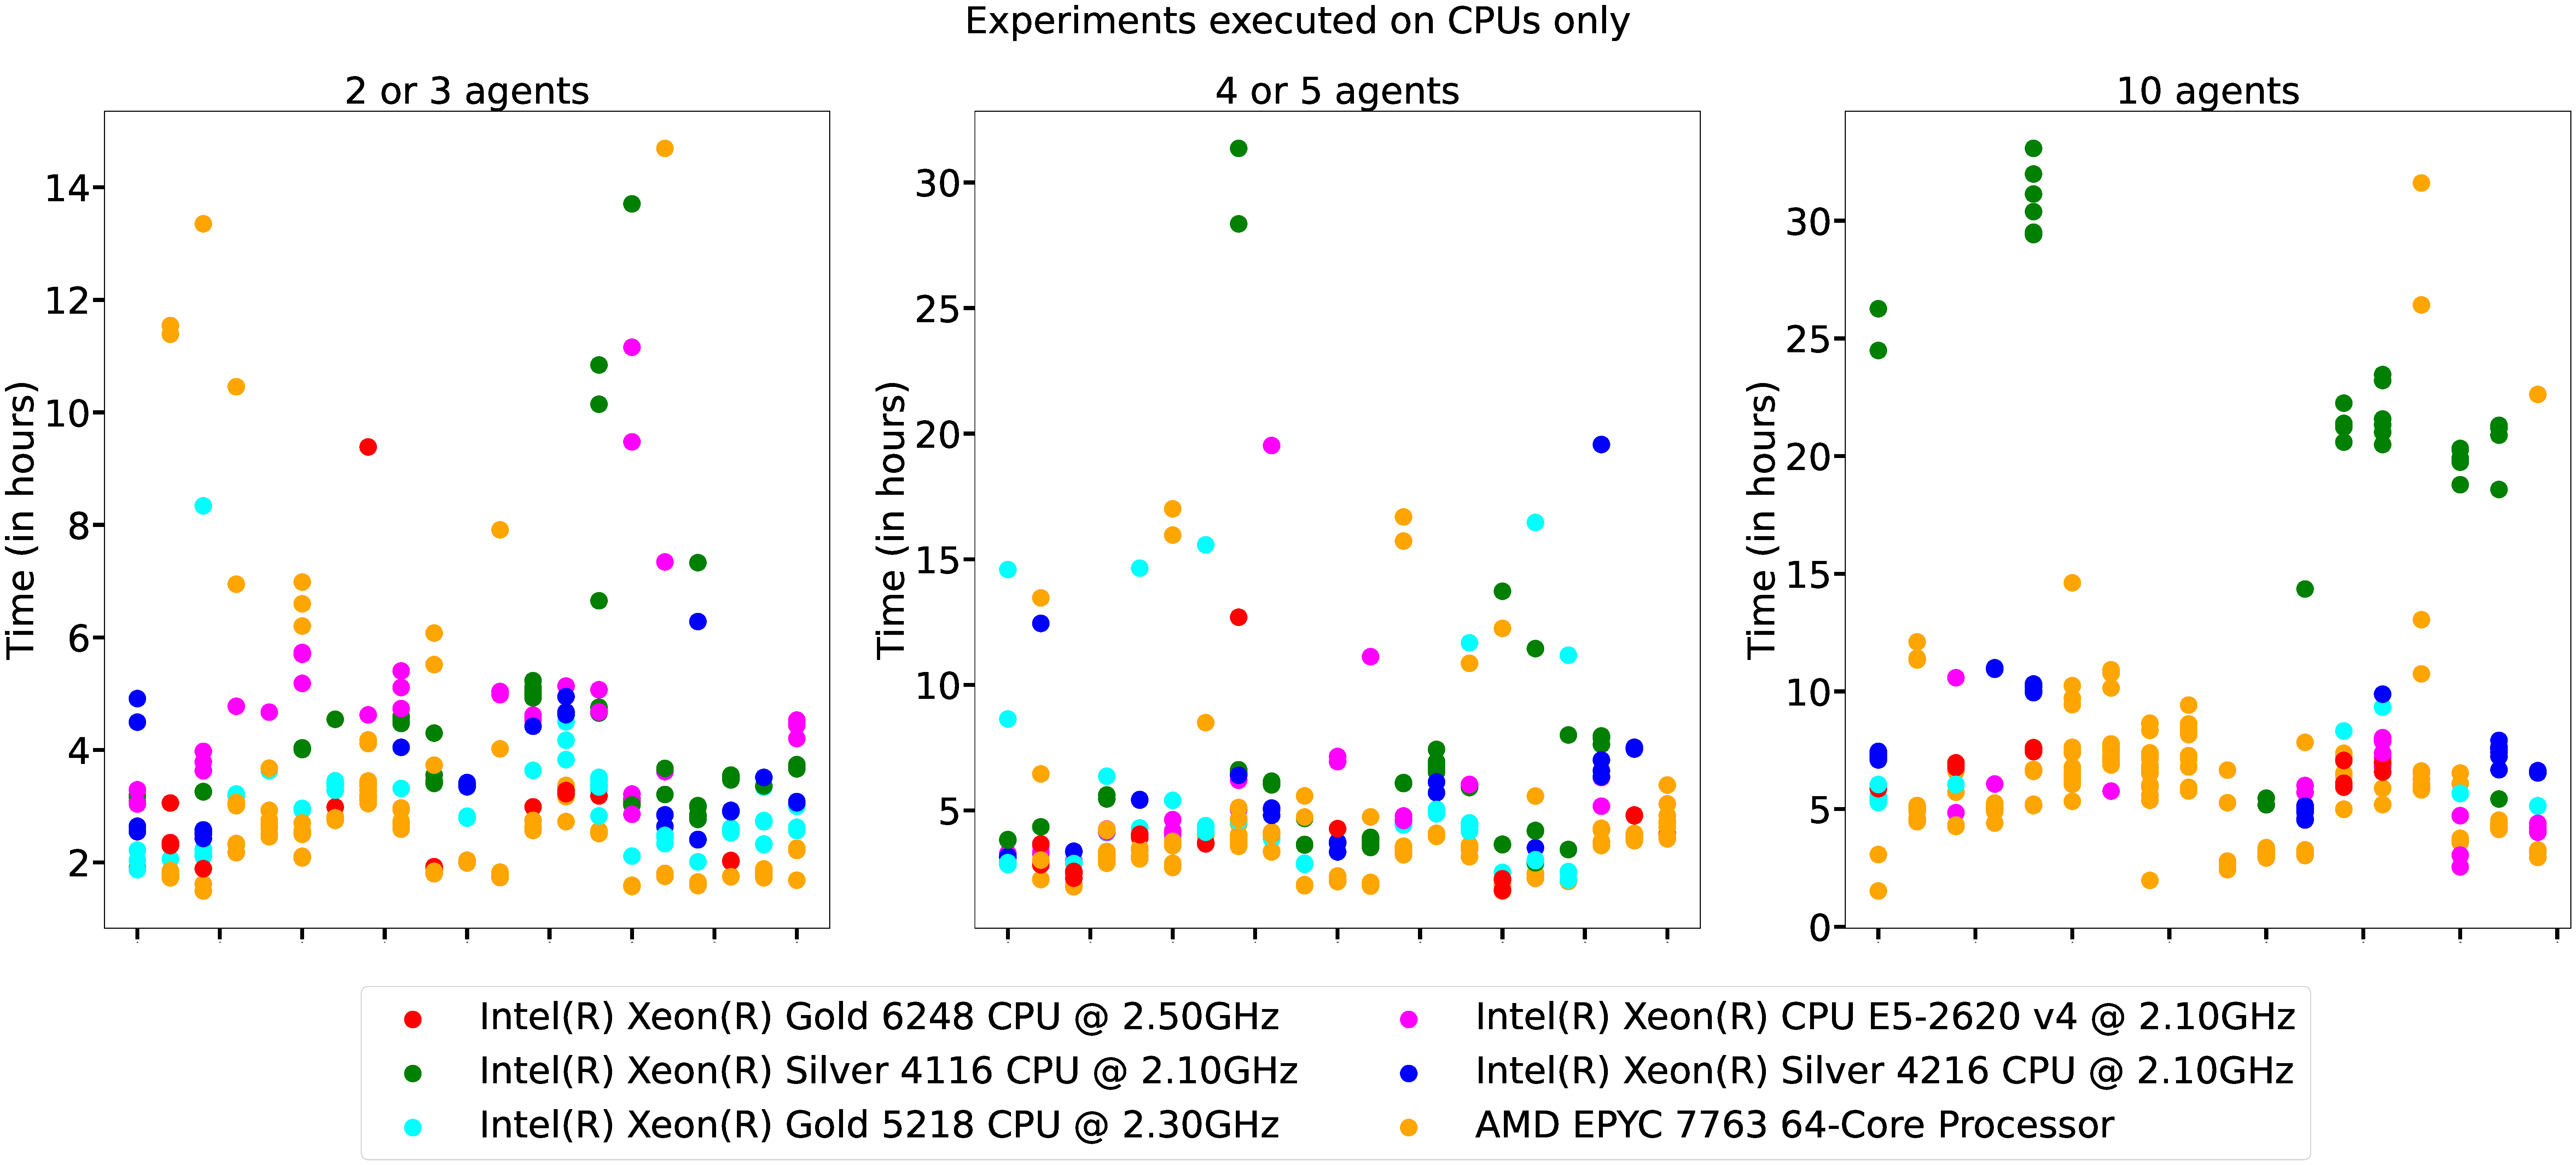
\includegraphics[width=\textwidth]{tex_thesis/figures/ch5/training_time_cpu.pdf}
    \caption{Training duration for experiments with $n<=10$ performed on only CPUs.}
    \label{fig:training_time_cpu}
\end{figure}

\begin{figure}
    \centering
    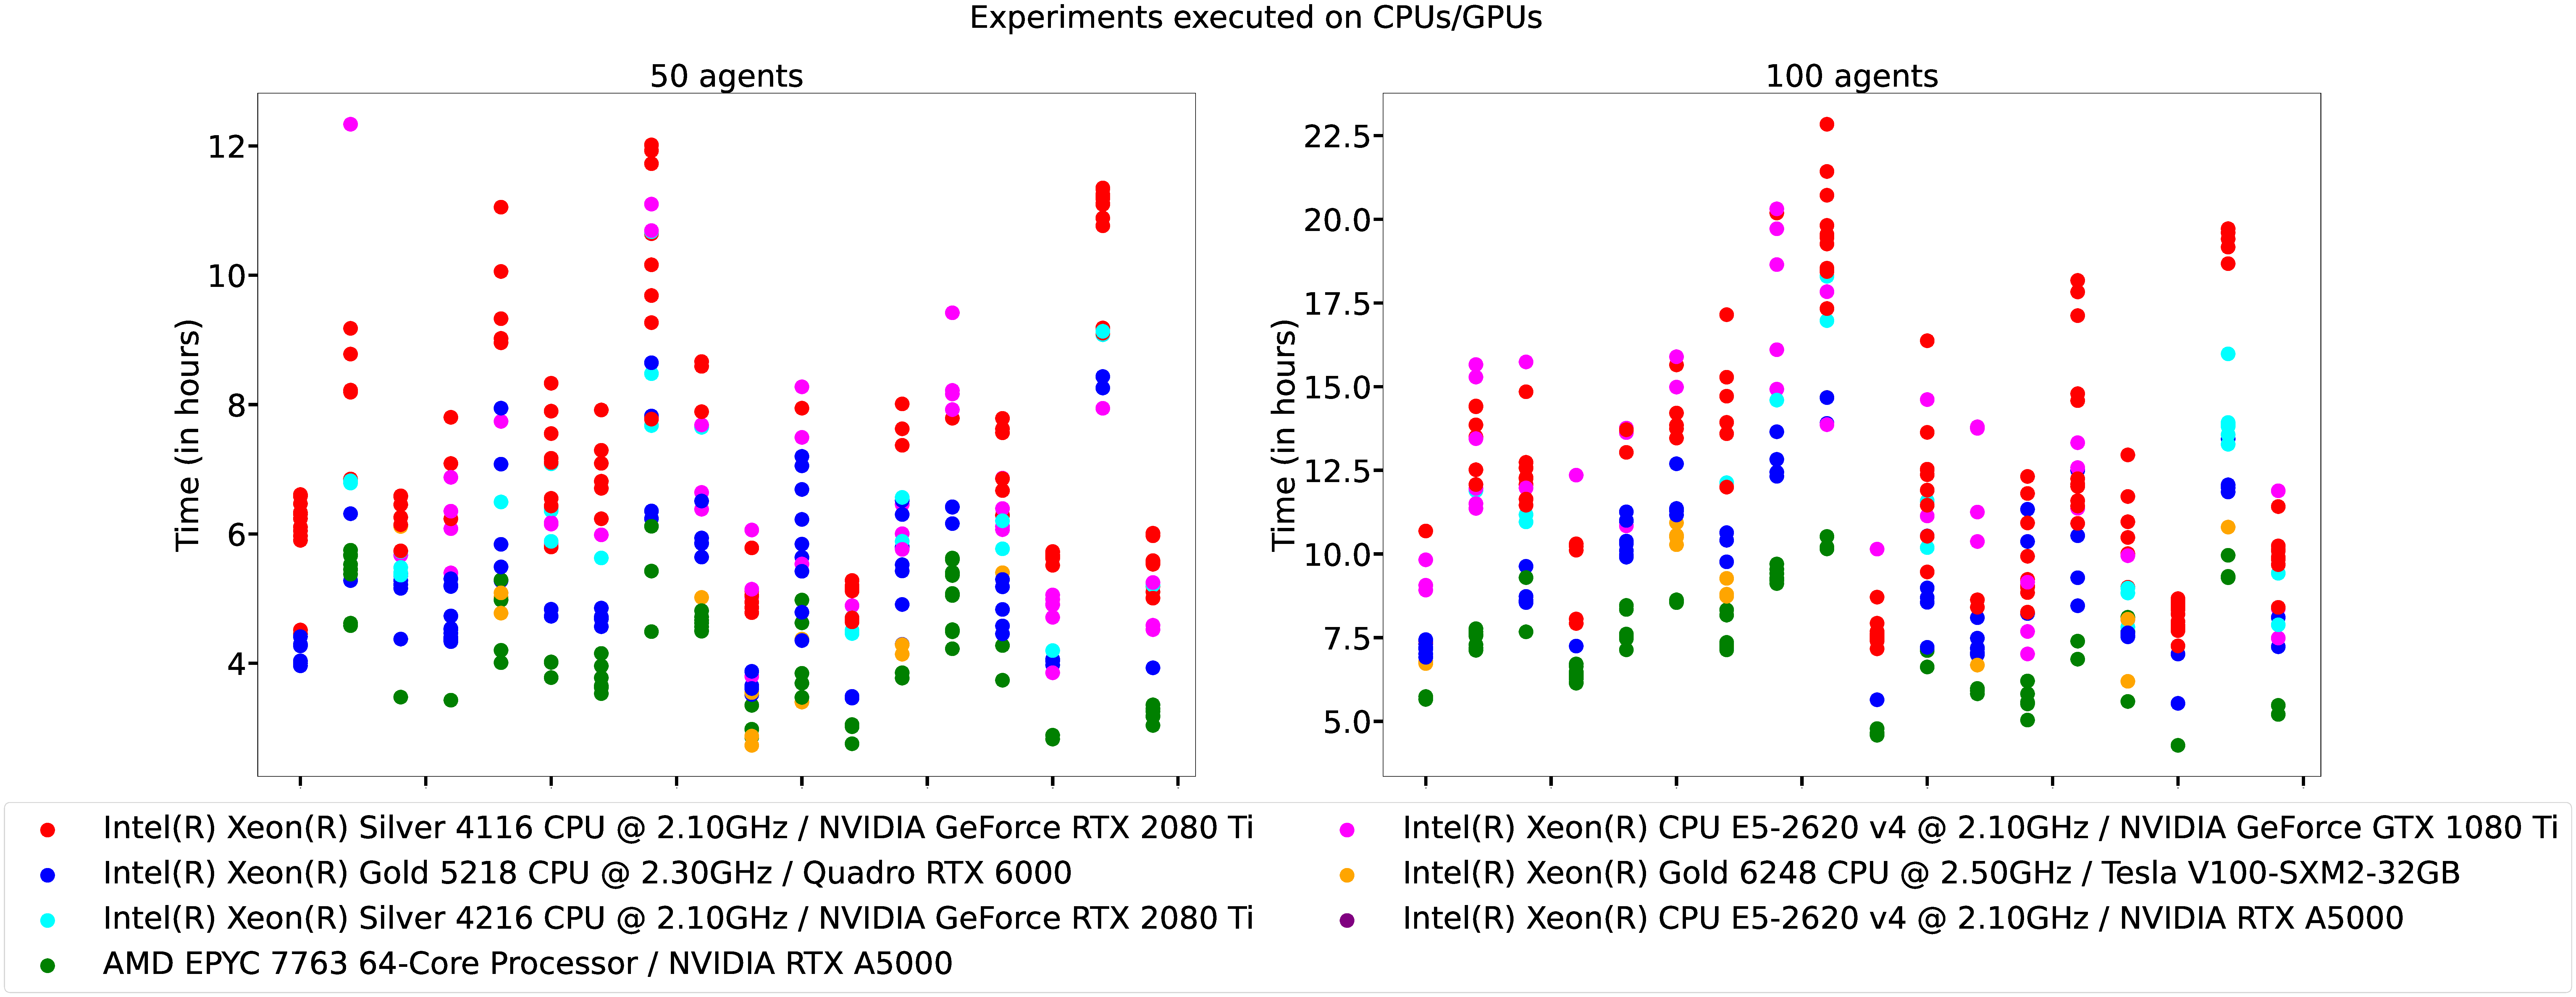
\includegraphics[width=\textwidth]{tex_thesis/figures/ch5/training_time_gpu.pdf}
    \caption{Training duration for experiments with $n>=50$ performed on CPUs and GPUs.}
    \label{fig:training_time_gpu}
\end{figure}

\begin{figure}
    \centering
    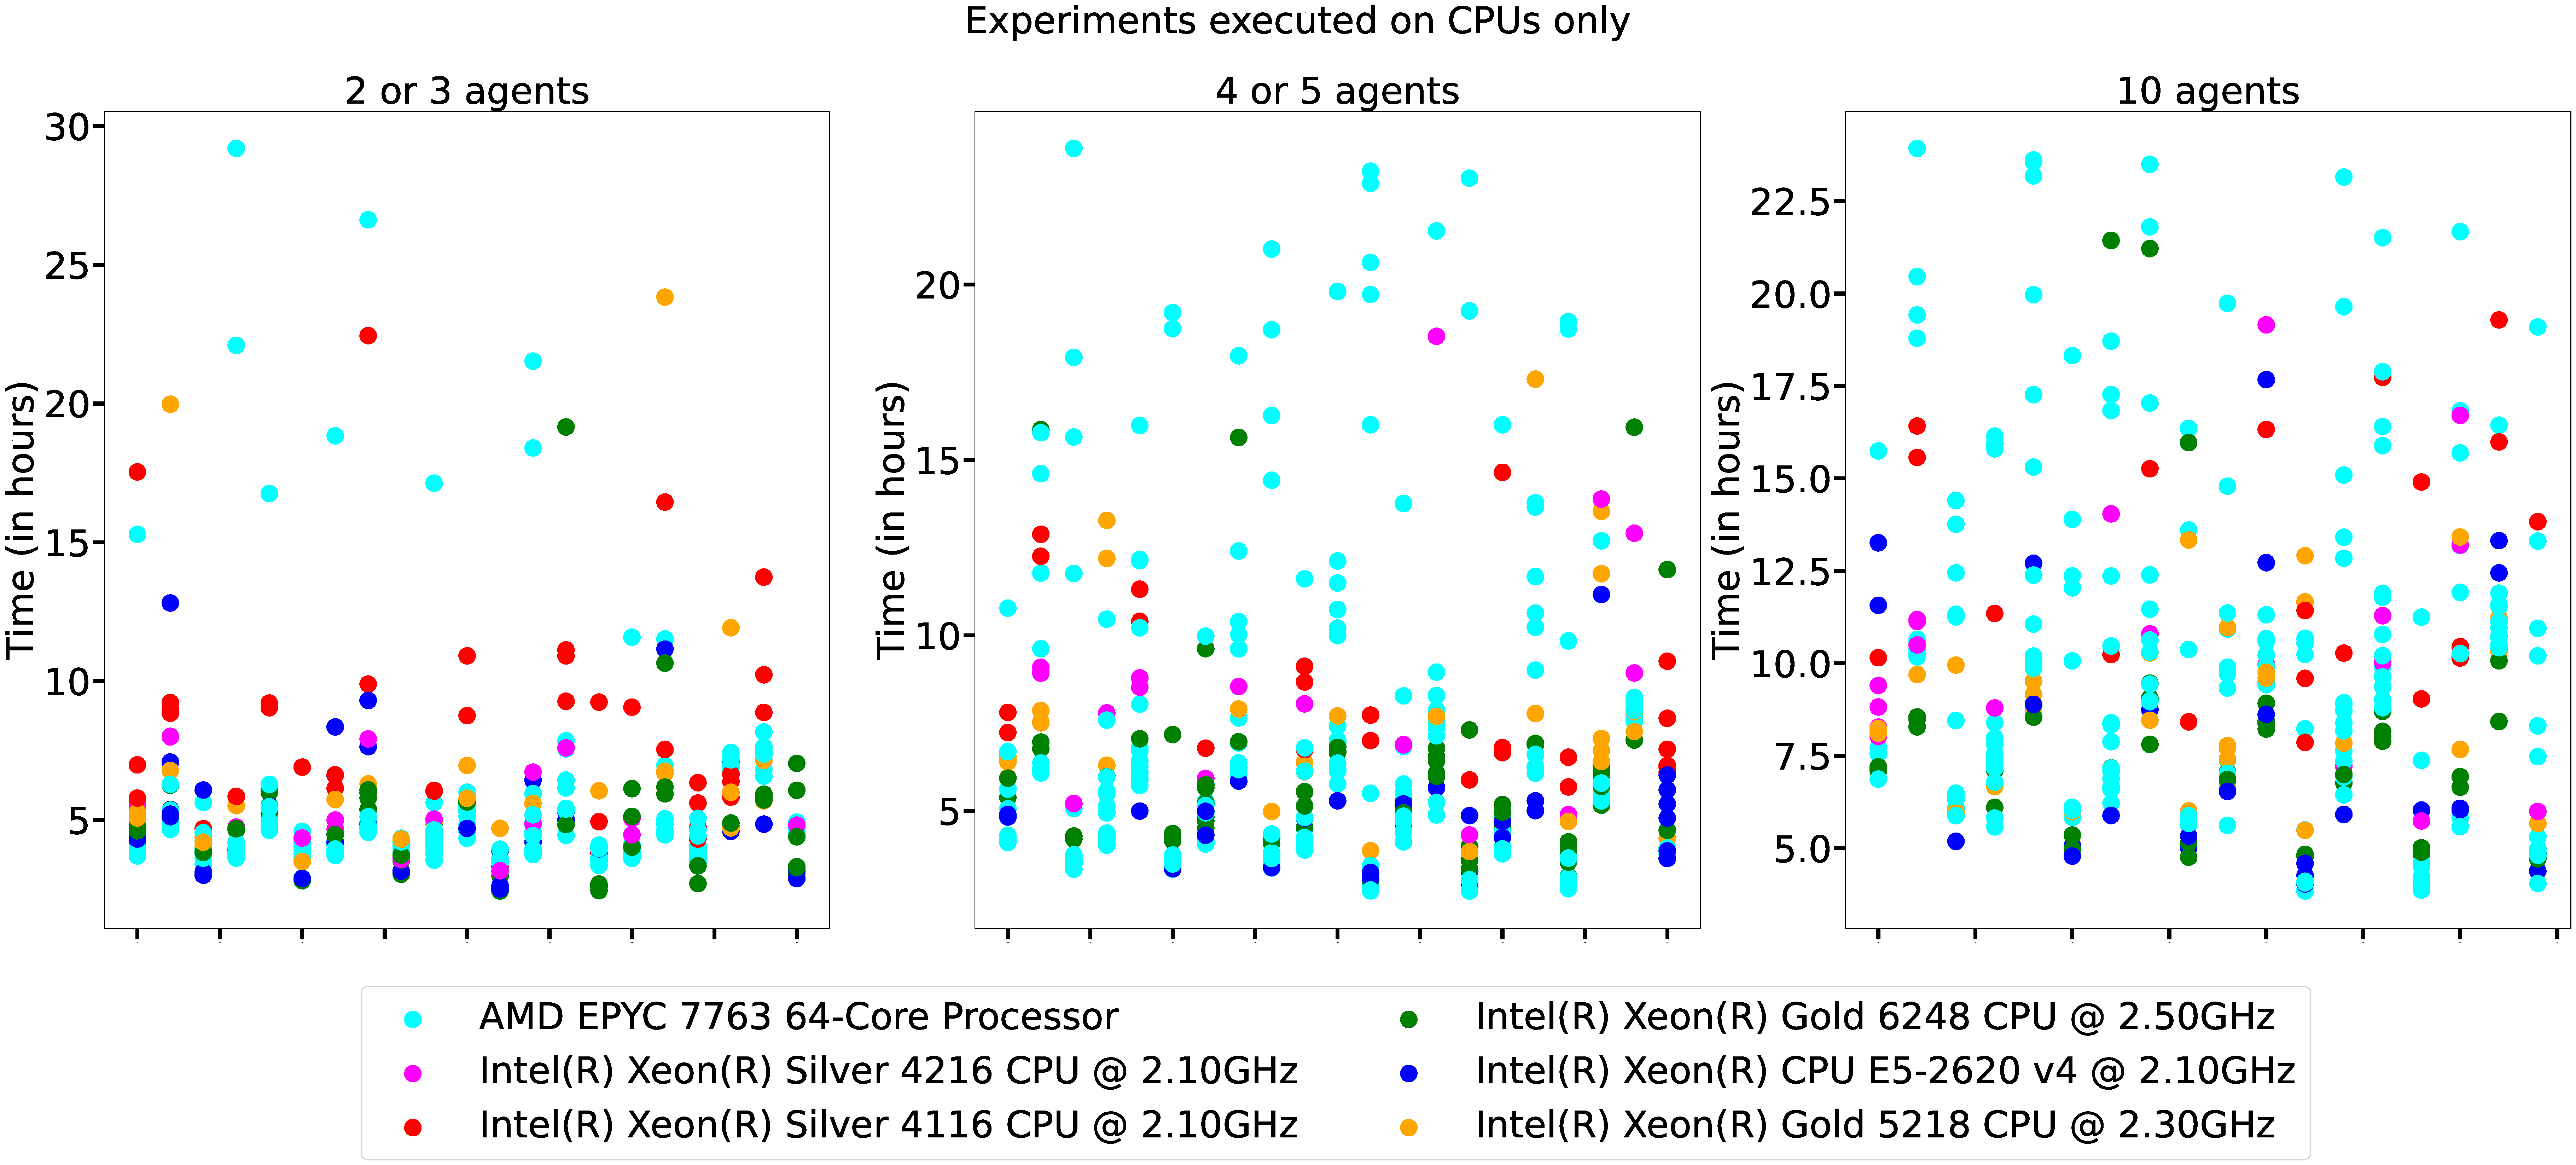
\includegraphics[width=\textwidth]{tex_thesis/figures/ch5/testing_time_cpu.pdf}
    \caption{Testing duration for experiments with $n<=10$ performed on only CPUs.}
    \label{fig:testing_time_cpu}
\end{figure}

\begin{figure}
    \centering
    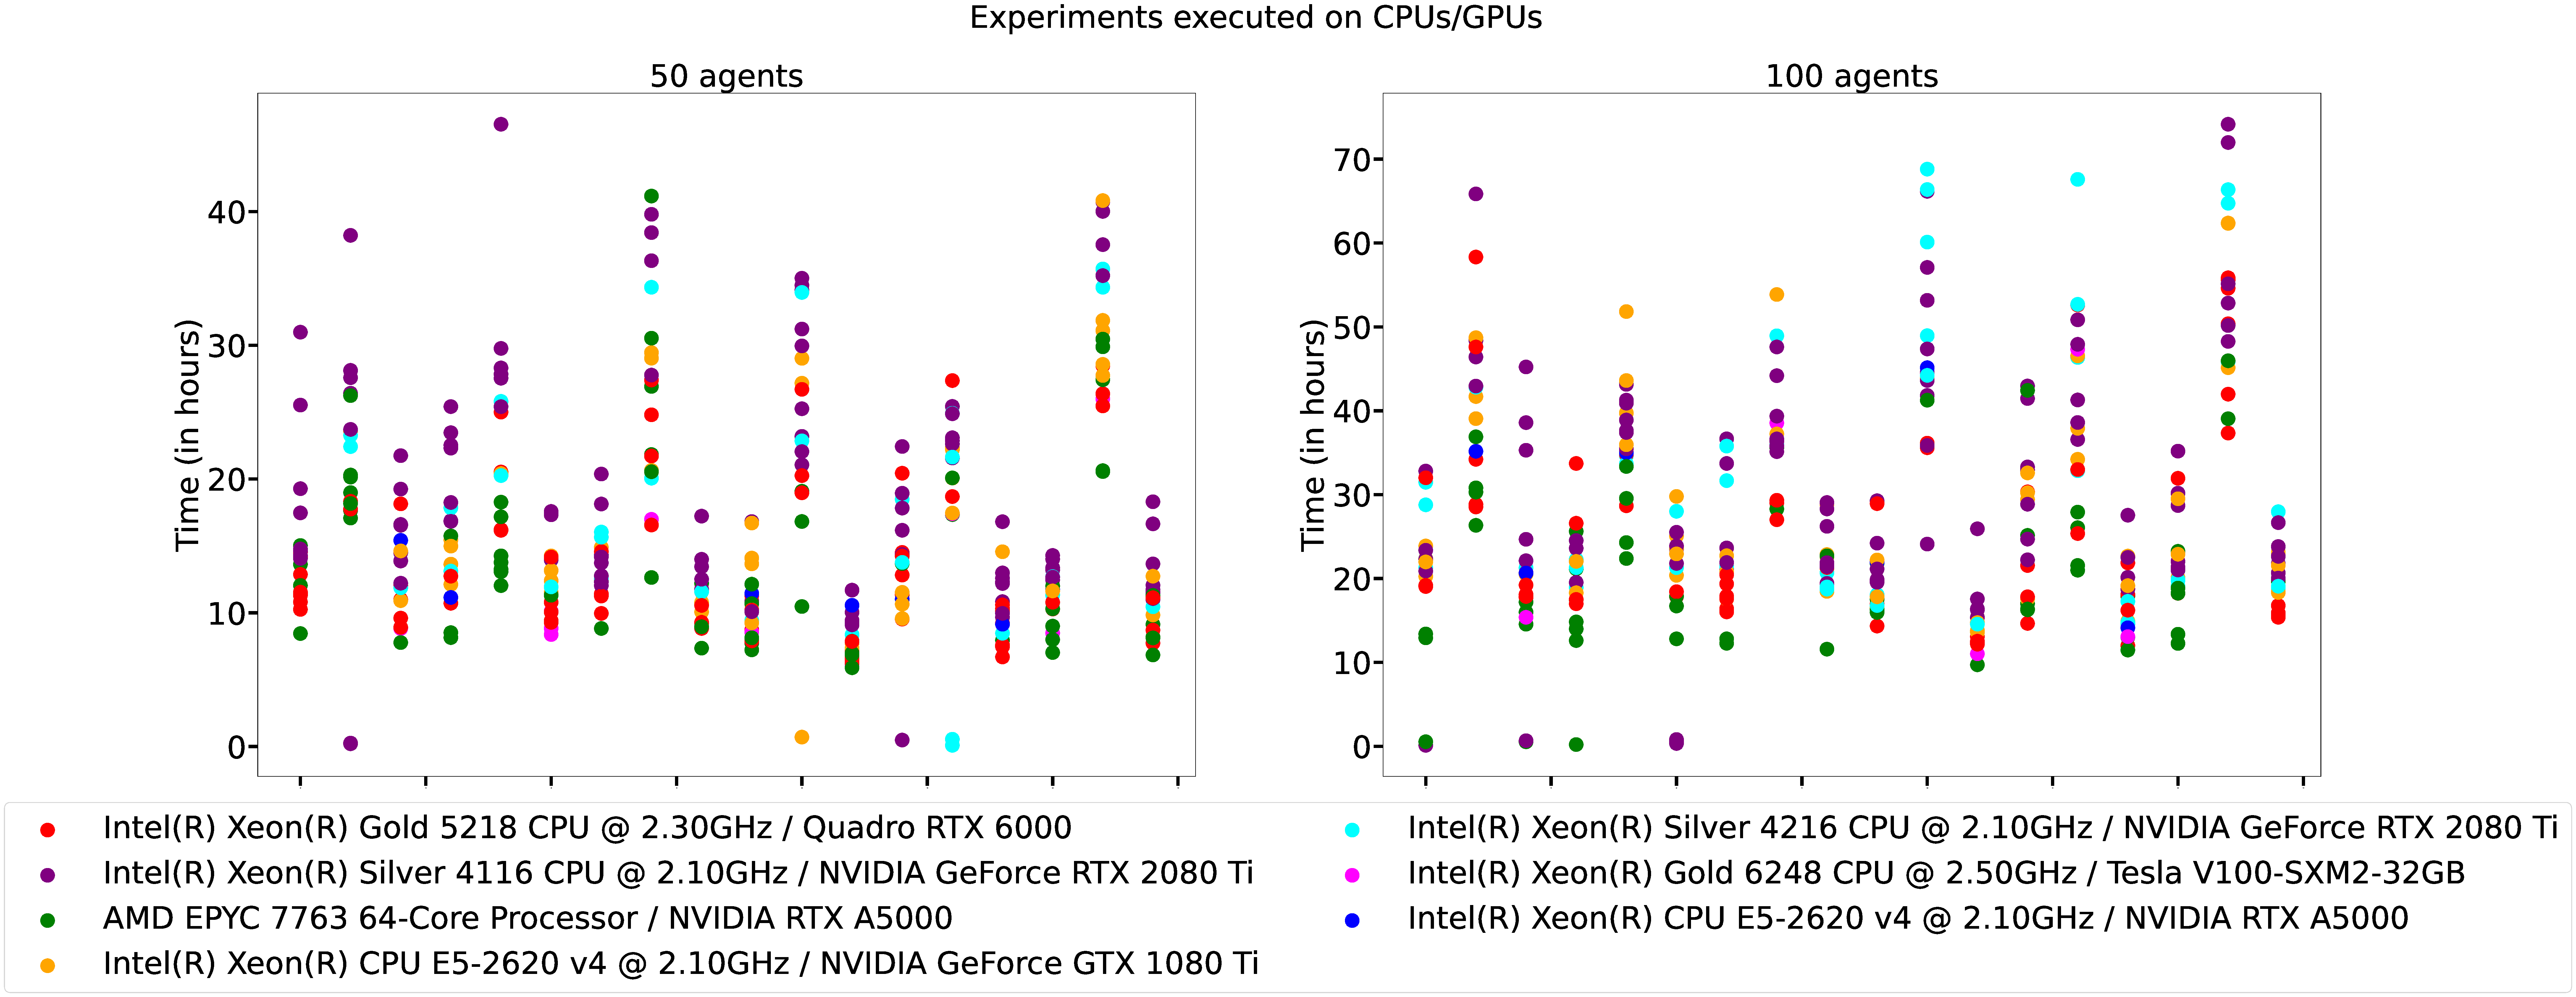
\includegraphics[width=\textwidth]{tex_thesis/figures/ch5/testing_time_gpu.pdf}
    \caption{Testing duration for experiments with $n>=50$ performed on CPUs and GPUs.}
    \label{fig:testing_time_gpu}
\end{figure}

The first observation that may be addressed is the resulting high variance. 
The variation across runs is logical because of the specific performance of the CPU/GPU models employed, but also due to the additional activity of clusters at the time of our experiments.
With respect to the computational time required for training, testing episodes are not executed and we can see that, by running the experiments on only CPUs, we manage to train the agents in less than $10$ hours, except for some occasional outliers.
For experiments with $50$ agents, and also relying on GPUs, the computational time is overall very similar to those previously mentioned, requiring less than $10$ hours, yet a longer time is needed for those with $100$ agents.
The fastest training results correspond to COMA because we are running four environments in parallel, instead of one during training.
We can see that IQL and QMIX follow closely, but QVMix, QPLEX, and FACMAC require additional computational time due to their architecture complexity.
Naturally, the testing stage needs more time compared to training for all experiments because it executes $10,000$ test episodes per stored network.
The correlated k-out-of-n environment slightly requires more time than the others because the correlation information is updated at every inspection step.


\begin{figure}
    \centering
    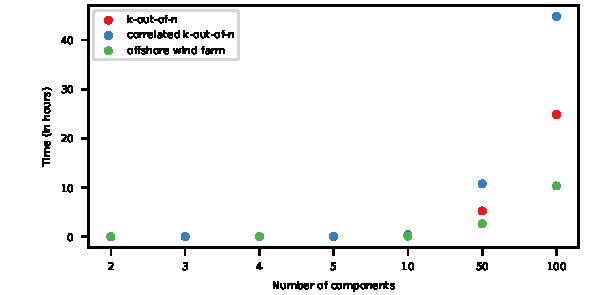
\includegraphics[width=.6\textwidth]{tex_thesis/figures/ch5/heur_cpu_time.pdf}
    \caption{Computational time required for executing expert-based heuristic policies as a function of the number of components. The experiments are run on 2 AMD EPYC Rome 7542 CPUs @ 2.9GHz.}
    \label{fig:heur_time_cpu}
\end{figure}
Furthermore, we represent in Figure \ref{fig:heur_time_cpu} the time required for the computation of expert-based heuristic policies. The experiments are plotted as a function of the number of components and coloured based on their corresponding environment. In this case, all experiments are run on CPUs. We can see that heuristic policies can be efficiently computed for environments with less than 50 components, yet the computational time significantly increases for experiments with 50 or 100 components. This result is logical since the combination of evaluated parameters includes the number of components to be inspected at each inspection interval. Besides, the overall computation time is directly influenced by the time needed to run an episode, with the k-out-of-n environments taking longer compared to the offshore wind farm ones because the episode's finite horizon spans over 10 additional time steps. 


\section{Additional benchmark results}
% All figures and detailed tables 
\label{sec:ch5_appendix_add_results}
In this section, we present additional results and remarks beyond those reported in the main text.
In the first place, we provide the values of the expected sum of discounted rewards achieved by the best runs over all experiments.
We list the best policy for each conducted experiment in Tables \ref{tab:koutofnresults}, \ref{tab:correlatedkoutofnresults}, and \ref{tab:owfresults}.
Note that the maximum values represented with markers at the right of each box in Figure \ref{fig:results} can be retrieved from these values by applying the normalisation (x-H)/H, with H being the value achieved by the heuristic policies.

Additionally, we represent in Figures \ref{fig:learning_curves_cc_false} and \ref{fig:learning_curves_cc_true} the learning curves corresponding to all our experiments.
The learning curves showcase the evolution of the expected sum of discounted rewards every 20,000 training time steps, computed at the testing stage with 10,000 test episodes.
Since the training is conducted with 10 different seeds for each environment and method, we also plot the corresponding 25th-75th percentiles around the median.
These results confirm the variance observed between the best results and presented in Figure \ref{fig:results}.

Based on Tables \ref{tab:koutofnresults} and \ref{tab:correlatedkoutofnresults}, one may additionally infer that correlated environments result in lower costs with respect to those uncorrelated.
This is especially true for environments with n>=10 agents, specified without campaign costs, and in all environments set up with campaign costs.
While MARL methods profit from the additionally provided correlation information, this is not always the case for the heuristic policies.

One final remark is that the discrepancy between the expert-based heuristic policy and MARL methods is more pronounced in offshore wind farm environments. 
This could be attributed to the shorter decision horizon or the higher cost per inspection in this particular case (see Table \ref{tab:owfresults}).

\newpage
\begin{table}
\centering
\caption{k-out-of-n system best policies (* = campaign cost).}
\label{tab:koutofnresults}
\setlength\tabcolsep{4.5pt}
\begin{tabular}{c|ccccccc|c}
\toprule
n & QMIX & QVMix & QPLEX & COMA & FACMAC & IQL & DQN & Heuristics \\
\midrule
3 & -9.7 & -9.8 & -9.7 & -10.6 & -10.4 & -35.3 & -9.9 & -12.5 \\
5 & -20.4 & -20.7 & -20.4 & -21.8 & -22.1 & -108.7 & -24.0 & -25.2 \\
10 & -51.0 & -51.5 & -51.0 & -54.3 & -61.3 & -404.5 & / & -63.7 \\
50 & -229.7 & -236.0 & -212.8 & -1190.6 & -249.0 & -1991.1 & / & -268.1 \\
100 & -222.6 & -230.7 & -220.6 & -1770.1 & -225.7 & -1770.1 & / & -262.4 \\
\midrule
*3 & -14.6 & -14.7 & -14.7 & -15.0 & -17.0 & -35.3 & -13.5 & -15.1 \\
*5 & -27.4 & -27.7 & -27.4 & -28.9 & -33.0 & -27.8 & -26.6 & -28.6 \\
*10 & -58.9 & -63.0 & -60.7 & -70.0 & -61.9 & -404.5 & / & -64.5 \\
*50 & -169.5 & -173.9 & -168.4 & -241.4 & -160.7 & -623.3 & / & -232.7 \\
*100 & -167.2 & -175.8 & -160.2 & -1770.1 & -144.8 & -1770.1 & / & -231.5 \\
\bottomrule
\end{tabular}
\end{table}



\begin{table}
\centering
\caption{Correlated k-out-of-n system best policies (* = campaign cost).}
\label{tab:correlatedkoutofnresults}
\setlength\tabcolsep{4.5pt}
\begin{tabular}{c|ccccccc|c}
\toprule
n & QMIX & QVMix & QPLEX & COMA & FACMAC & IQL & DQN & Heuristics \\
\midrule
3 & -9.7 & -9.7 & -9.6 & -11.0 & -10.6 & -10.0 & -10.0 & -13.0 \\
5 & -20.4 & -20.6 & -18.4 & -21.2 & -21.6 & -20.2 & -23.4 & -28.1 \\
10 & -47.6 & -51.0 & -45.2 & -49.7 & -46.1 & -374.5 & / & -67.7 \\
50 & -214.3 & -233.0 & -212.3 & -419.3 & -143.4 & -1339.9 & / & -240.0 \\
100 & -250.3 & -289.0 & -276.8 & -486.9 & -118.3 & -1744.0 & / & -218.1 \\
\midrule
*3 & -13.1 & -12.9 & -12.9 & -14.8 & -18.0 & -34.7 & -12.6 & -15.2 \\
*5 & -23.5 & -24.7 & -23.5 & -28.2 & -29.2 & -23.9 & -26.8 & -30.5 \\
*10 & -56.2 & -53.4 & -50.1 & -52.8 & -49.2 & -56.0 & / & -68.5 \\
*50 & -132.6 & -157.1 & -121.2 & -159.3 & -106.6 & -814.9 & / & -211.0 \\
*100 & -147.7 & -147.5 & -121.0 & -339.1 & -71.3 & -723.8 & / & -194.0 \\
\bottomrule
\end{tabular}
\end{table}



\begin{table}
\centering
\caption{Offshore wind farm best policies (* = campaign cost).}
\label{tab:owfresults}
\setlength\tabcolsep{4.5pt}
\begin{tabular}{c|ccccccc|c}
\toprule
n & QMIX & QVMix & QPLEX & COMA & FACMAC & IQL & DQN & Heuristics \\
\midrule
2 & -23.3 & -23.3 & -23.2 & -23.7 & -40.5 & -23.7 & -23.2 & -58.3 \\
4 & -47.1 & -47.4 & -47.1 & -47.9 & -122.4 & -47.4 & -47.7 & -116.9 \\
10 & -118.4 & -119.4 & -118.5 & -122.2 & -235.2 & -120.8 & / & -292.3 \\
50 & -604.4 & -613.9 & -604.6 & -2805.8 & -627.3 & -2892.5 & / & -1463.8 \\
100 & -1224.1 & -1238.8 & -1213.2 & -5785.1 & -1625.2 & -5785.1 & / & -2925.0 \\
\midrule
*2 & -51.8 & -52.0 & -51.9 & -60.1 & -60.3 & -52.0 & -48.9 & -62.2 \\
*4 & -80.5 & -80.7 & -80.7 & -122.2 & -118.6 & -85.6 & -76.0 & -115.2 \\
*10 & -129.3 & -133.3 & -130.0 & -314.5 & -196.4 & -132.0 & / & -267.2 \\
*50 & -432.9 & -436.9 & -434.5 & -2892.5 & -502.8 & -1709.7 & / & -1248.2 \\
*100 & -808.1 & -829.0 & -852.3 & -5785.1 & -1280.5 & -5785.1 & / & -2436.3 \\
\bottomrule
\end{tabular}
\end{table}


\begin{figure*}

\includegraphics[width=\textwidth]{tex_thesis/figures/ch5/all_3_cc_False.pdf}

\includegraphics[width=\textwidth]{tex_thesis/figures/ch5/all_5_cc_False.pdf}

\includegraphics[width=\textwidth]{tex_thesis/figures/ch5/all_10_cc_False.pdf}

\includegraphics[width=\textwidth]{tex_thesis/figures/ch5/all_50_cc_False.pdf}

\includegraphics[width=\textwidth]{tex_thesis/figures/ch5/all_100_cc_False.pdf}
\caption{
Learning curves in all environments with no campaign cost. 
Curves represent the sum of discounted rewards obtained during test time.
The bold line is the median while the error bands are delimited by the 25th and 75th percentiles.
Colours represent the different methods and the parameters of each environment can be inferred from the title above its corresponding graph.
}
    \label{fig:learning_curves_cc_false}
\end{figure*}

\begin{figure*}

\includegraphics[width=\textwidth]{tex_thesis/figures/ch5/all_3_cc_True.pdf}

\includegraphics[width=\textwidth]{tex_thesis/figures/ch5/all_5_cc_True.pdf}

\includegraphics[width=\textwidth]{tex_thesis/figures/ch5/all_10_cc_True.pdf}

\includegraphics[width=\textwidth]{tex_thesis/figures/ch5/all_50_cc_True.pdf}

\includegraphics[width=\textwidth]{tex_thesis/figures/ch5/all_100_cc_True.pdf}
\caption{
Learning curves in all environments with campaign cost. 
Curves represent the sum of discounted rewards obtained during test time.
The bold line is the median while the error bands are delimited by the 25th and 75th percentiles.
Colours represent the different methods and the parameters of each environment can be inferred from the title above its corresponding graph.
}
\label{fig:learning_curves_cc_true}
\end{figure*}

